\section{E2: Traffic with an obstacle}
\newcommand{\Ex}{E2}
The previous experiment demonstrated the performance of our proposed GM-PHD filter method, which incorporated
the dynamic detection probability and the modified pruning. Our method has proven superior to the standard
GM-PHD
filter with the constant
detection probability. Nevertheless, our method was primarily designed to excel in situations where obstacles obscure camera views. To assess its effectiveness in such scenarios, we propose Experiment \textit{E2}.

\subsection{V3}
\newcommand{\Vs}{V3}
In the video \textit{V3} a light pole is in the camera's view, preventing the object detector to detect hidden objects. The
frame rate of this video is set to 10 fps.

\subsection{V3 - GM-PHD with the constant detection probability}
\newcommand{\Set}{S0}
The targets cannot persist beyond a certain number of time steps without being measured, resulting in their loss once they surpass an obstacle. To avert a permanent loss, a new spawning point is introduced immediately after the obstacle to revive the lost target. However, this approach comes with a drawback: the revived target starts afresh without retaining its previous history.

Parameter settings are embodied in Table \ref{tab:\Ex-\Vs-\Set}.

\begin{table}[!h]
    \centering
    \begin{tabular}{|c|c|c|c|c|c|}
        \hline
        $P_{D}$ & $P$ & $\sigma_{\upsilon}$ & $\sigma_{\epsilon}$ & $T_p$ & $T_{YOLO}$ \\ \noalign{\hrule height 1.5pt}
        0.9 & $diag(500,500,500,500)$ & 0.1 & 100 & 0.1 & 0.3\\
        \hline
    \end{tabular}
    \caption{The parameter settings for Experiment {\Ex-\Vs} with the constant detection probability.}
    \label{tab:\Ex-\Vs-\Set}
\end{table}

Figure \ref{fig:\Ex-\Vs-\Set} shows some highlights of the GM-PHD filter with the constant detection probability.
\begin{itemize}
    \item \textbf{\ref{fig:\Ex-\Vs-\Set:01}:} The sequence starts with the frame no. 7. The first car is initiaized by
    the spawning point.
    \item \textbf{\ref{fig:\Ex-\Vs-\Set:02}:} The first car arrives to an obstacle. Meanwhile, the second car arrives.
    \item \textbf{\ref{fig:\Ex-\Vs-\Set:03}:} The YOLO object detector is not able to detect the hidden car. The target is removed.
    \item \textbf{\ref{fig:\Ex-\Vs-\Set:04}:} The previously lost target is detected and initialized due to the
    second spawning point. Nevertheless, the history of this target is still lost. Moreover, the target has not been tracked for five consecutive frames.
    \item \textbf{\ref{fig:\Ex-\Vs-\Set:05}:} The second car is not detected due to the obstacle. The track of the target is lost.
    \item \textbf{\ref{fig:\Ex-\Vs-\Set:06}:} The target is once again initialized by the second spawning point. The
    third car approaches the first spawning point.
    \item \textbf{\ref{fig:\Ex-\Vs-\Set:07}:} The last car is also not detected behind the obstacle, thus its track is lost.
    \item \textbf{\ref{fig:\Ex-\Vs-\Set:08}:} Even though the target is reborn, the track of this target has not been
    available for 6 frames in a row. The other two cars are further away and appear to be in the same neighbourhood.
    The filter merged these two targets into a single one.
\end{itemize}

According to Graph \ref{gr:\Ex-\Vs-\Set}, the filter is able to track the targets admirably. However, the graph also
shows the weakness of this approach. The peaks displaying the target's loss are clearly present.

With the second spawn point enabling targets to reborn, the GM-PHD filter is able to track all the targets accurately.
The weakness of this approach is definite -- if a target is reborn, it is a whole new target without any history.

\begin{figure}[H]
    \centering
    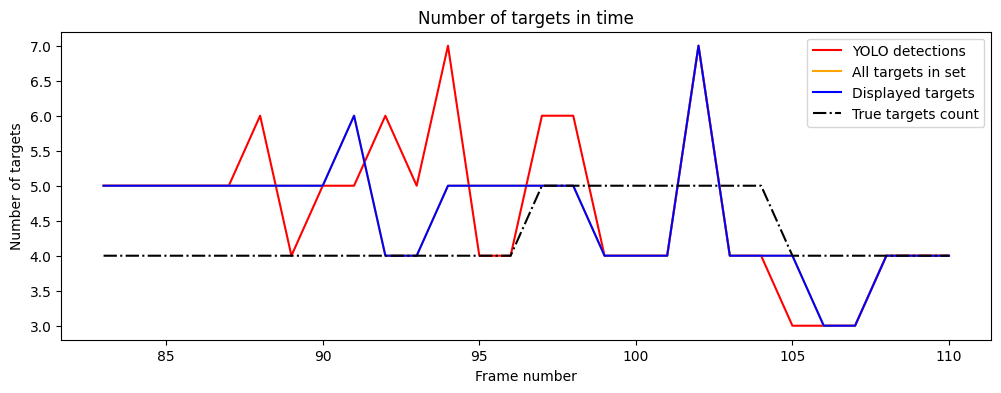
\includegraphics[width=\linewidth]{../../../experiments/\Ex/\Vs/noPd/staticPd_det}
    \caption{Development chart of the number of detected targets, targets in the filter's queue, displayed targets and
    true targets' count.}
    \label{gr:\Ex-\Vs-\Set}
\end{figure}

\begin{figure}[H]
    \centering
    \begin{subfigure}{0.23\textwidth}
        \centering
        \includegraphics[width=\linewidth]{../../../experiments/\Ex/\Vs/noPd/7}
        \caption{Frame number: 7.}
        \label{fig:\Ex-\Vs-\Set:01}
    \end{subfigure}
    \begin{subfigure}{0.23\textwidth}
        \centering
        \includegraphics[width=\linewidth]{../../../experiments/\Ex/\Vs/noPd/33}
        \caption{Frame number: 33.}
        \label{fig:\Ex-\Vs-\Set:02}
    \end{subfigure}
    \begin{subfigure}{0.23\textwidth}
        \centering
        \includegraphics[width=\linewidth]{../../../experiments/\Ex/\Vs/noPd/38}
        \caption{Frame number: 38.}
        \label{fig:\Ex-\Vs-\Set:03}
    \end{subfigure}
    \begin{subfigure}{0.23\textwidth}
        \centering
        \includegraphics[width=\linewidth]{../../../experiments/\Ex/\Vs/noPd/43}
        \caption{Frame number: 43.}
        \label{fig:\Ex-\Vs-\Set:04}
    \end{subfigure}
    \\
    \begin{subfigure}{0.23\textwidth}
        \centering
        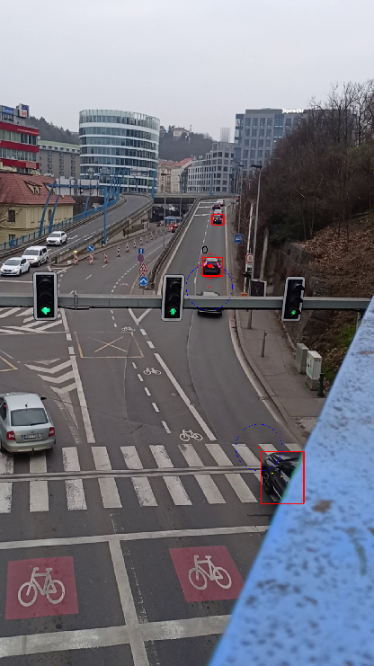
\includegraphics[width=\linewidth]{../../../experiments/\Ex/\Vs/noPd/55}
        \caption{Frame number: 55.}
        \label{fig:\Ex-\Vs-\Set:05}
    \end{subfigure}
    \begin{subfigure}{0.23\textwidth}
        \centering
        \includegraphics[width=\linewidth]{../../../experiments/\Ex/\Vs/noPd/60}
        \caption{Frame number: 60.}
        \label{fig:\Ex-\Vs-\Set:06}
    \end{subfigure}
    \begin{subfigure}{0.23\textwidth}
        \centering
        \includegraphics[width=\linewidth]{../../../experiments/\Ex/\Vs/noPd/85}
        \caption{Frame number: 85.}
        \label{fig:\Ex-\Vs-\Set:07}
    \end{subfigure}
    \begin{subfigure}{0.23\textwidth}
        \centering
        \includegraphics[width=\linewidth]{../../../experiments/\Ex/\Vs/noPd/92}
        \caption{Frame number: 92.}
        \label{fig:\Ex-\Vs-\Set:08}
    \end{subfigure}
    \caption{Image sequence of tracked objects using the GM-PHD filter with the constant detection probability.}
    \label{fig:\Ex-\Vs-\Set}
\end{figure}




\subsection{V3 -- GM-PHD with the dynamic detection probability}
Experiments using the video \textit{V3} utilizing the GM-PHD filter with the dynamic detection probability and
settings \textit{S1, S2,
    S3} are
demonstrated in following sections.
\subsubsection{S1 -- YOLO + YOLO}
\renewcommand{\Set}{S1}
This experiment uses settings \textit{S1}, where the YOLO model provides both object detection bboxes and
segmentation masks.
The parameter settings are shown in Table \ref{tab:\Ex-\Vs-\Set}.
\begin{table}[H]
    \centering
    \begin{tabular}{|c|c|c|c|c|c|c|c|c|}
        \hline
        $P_{D,k}(x)$ & $P$ & $\sigma_{\upsilon}$ & $\sigma_{\epsilon}$ & $T_H$ & $T_d$ & $T_p$ & $T_l$ & $T_{YOLO}$ \\ \noalign{\hrule
        height 1.5pt}
        0.3 & $diag(500,500,500,500)$ & 0.1 & 100 & 2 & 3 & 0.1 & 0.0001 & 0.3\\
        \hline
    \end{tabular}
    \caption{The parameter settings for Experiment {\Ex-\Vs-\Set} with the dynamic detection probability.}
    \label{tab:\Ex-\Vs-\Set}
\end{table}

Figure \ref{fig:\Ex-\Vs-\Set} shows the performance of the GM-PHD filter with the dynamic detection probability with settings \textit{S1}.
\begin{itemize}
    \item \textbf{\ref{fig:\Ex-\Vs-\Set:01}:} The tracking starts with frame no. 7. The first target approaches the spawning point.
    \item \textbf{\ref{fig:\Ex-\Vs-\Set:02}:} The first car reaches the light pole. The second car appears in the scene.
    \item \textbf{\ref{fig:\Ex-\Vs-\Set:03}:} The first car is detected by YOLO for the last time before
    temporarily disappearing
    behind the obstacle.
    \item \textbf{\ref{fig:\Ex-\Vs-\Set:04}:} Even though the first car has not been detected for 5 frames, it is able
    to survive without the second spawning point.
    \item \textbf{\ref{fig:\Ex-\Vs-\Set:05}:} In this frame, an example of the \textit{hidden} target's state can be
    seen. The second car is annotated with number 1, i.e., it is considered as hidden.
    \item \textbf{\ref{fig:\Ex-\Vs-\Set:06}:} The second car overcomes the obstacle and continues in its path. This target was able to survive for 6 consecutive time steps.
    \item \textbf{\ref{fig:\Ex-\Vs-\Set:07}:} As the two cars appear close to each other, more measurements appear in
    the validation region of the targets. The third car is not detected behind the light pole, but is still tracked.
    \item \textbf{\ref{fig:\Ex-\Vs-\Set:08}:} The first two cars' targets are merged together, due to the long distance
    from the camera, static motion and observation noises. The third target also survives the misdetection period.
\end{itemize}

The displayed targets line in Graph \ref{gr:\Ex-\Vs-\Set} is almost the same as in previous experiment. However, the
orange line shows, that the filter is still informed about all potential targets. As seen in \ref{fig:\Ex-\Vs-\Set} the hidden targets are not lost, their weights are just too small to be displayed.

The performance of the GM-PHD filter with the dynamic detection probability might seem to be very similar to the
constant detection probability at first glance. But the targets are not removed when hidden. Moreover, the targets' track history is not lost.

\begin{figure}[H]
    \centering
    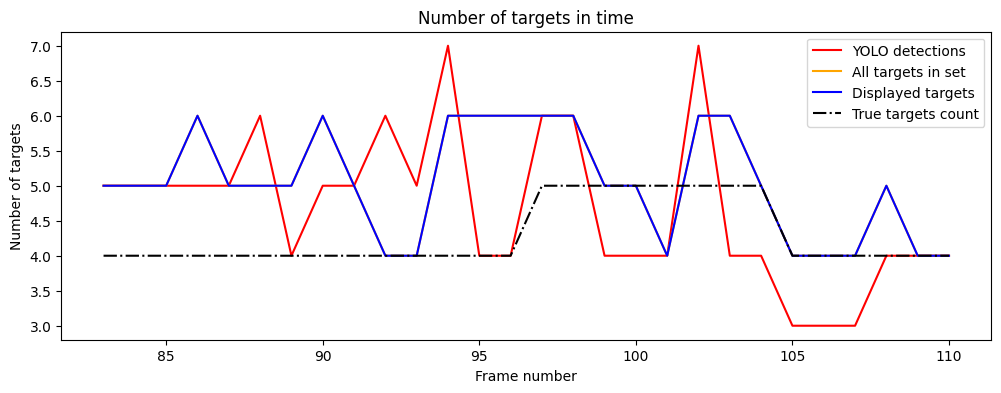
\includegraphics[width=\linewidth]{../../../experiments/\Ex/\Vs/YOLO/yolo_det}
    \caption{Development chart of the number of detected targets, targets in the filter's queue, displayed targets and
    true targets' count.}
    \label{gr:\Ex-\Vs-\Set}
\end{figure}

\begin{figure}[H]
    \centering
    \begin{subfigure}{0.23\textwidth}
        \centering
        \includegraphics[width=\linewidth]{../../../experiments/\Ex/\Vs/YOLO/7}
        \caption{Frame number: 7.}
        \label{fig:\Ex-\Vs-\Set:01}
    \end{subfigure}
    \begin{subfigure}{0.23\textwidth}
        \centering
        \includegraphics[width=\linewidth]{../../../experiments/\Ex/\Vs/YOLO/33}
        \caption{Frame number: 33.}
        \label{fig:\Ex-\Vs-\Set:02}
    \end{subfigure}
    \begin{subfigure}{0.23\textwidth}
        \centering
        \includegraphics[width=\linewidth]{../../../experiments/\Ex/\Vs/YOLO/38}
        \caption{Frame number: 38.}
        \label{fig:\Ex-\Vs-\Set:03}
    \end{subfigure}
    \begin{subfigure}{0.23\textwidth}
        \centering
        \includegraphics[width=\linewidth]{../../../experiments/\Ex/\Vs/YOLO/43}
        \caption{Frame number: 43.}
        \label{fig:\Ex-\Vs-\Set:04}
    \end{subfigure}
    \\
    \begin{subfigure}{0.23\textwidth}
        \centering
        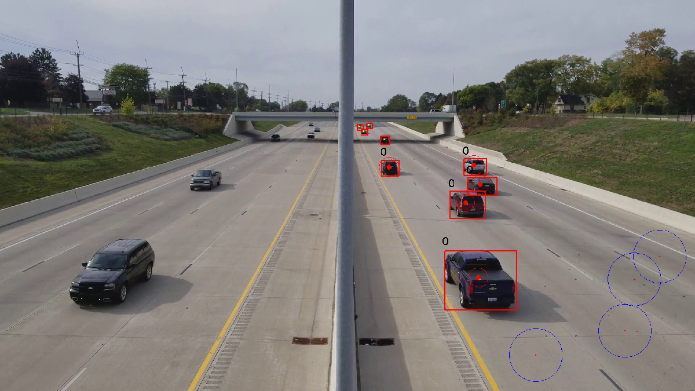
\includegraphics[width=\linewidth]{../../../experiments/\Ex/\Vs/YOLO/58}
        \caption{Frame number: 58.}
        \label{fig:\Ex-\Vs-\Set:05}
    \end{subfigure}
    \begin{subfigure}{0.23\textwidth}
        \centering
        \includegraphics[width=\linewidth]{../../../experiments/\Ex/\Vs/YOLO/60}
        \caption{Frame number: 60.}
        \label{fig:\Ex-\Vs-\Set:06}
    \end{subfigure}
    \begin{subfigure}{0.23\textwidth}
        \centering
        \includegraphics[width=\linewidth]{../../../experiments/\Ex/\Vs/YOLO/85}
        \caption{Frame number: 85.}
        \label{fig:\Ex-\Vs-\Set:07}
    \end{subfigure}
    \begin{subfigure}{0.23\textwidth}
        \centering
        \includegraphics[width=\linewidth]{../../../experiments/\Ex/\Vs/YOLO/92}
        \caption{Frame number: 92.}
        \label{fig:\Ex-\Vs-\Set:08}
    \end{subfigure}
    \caption{Image sequence of tracked objects using the GM-PHD filter with the dynamic detection probability and YOLO
    only.}
    \label{fig:\Ex-\Vs-\Set}
\end{figure}




\subsubsection{S2 -- YOLO + SAM}
\renewcommand{\Set}{S2}
The next settings employs settings \textit{S2} with the YOLO object detector and the SAM
segmentation model on the video \textit{V3}.
All parameters are included in Table \ref{tab:\Ex-\Vs-\Set}.
\begin{table}[H]
    \centering
    \begin{tabular}{|c|c|c|c|c|c|c|c|c|}
        \hline
        $P_{D,k}(x)$ & $P$ & $\sigma_{\upsilon}$ & $\sigma_{\epsilon}$ & $T_H$ & $T_d$ & $T_p$ & $T_l$ & $T_{YOLO}$ \\ \noalign{\hrule
        height 1.5pt}
        0.3 & $diag(500,500,500,500)$ & 0.1 & 100 & 2 & 3 & 0.1 & 0.0001 & 0.3\\
        \hline
    \end{tabular}
    \caption{The parameter settings for Experiment {\Ex-\Vs-\Set} with the dynamic detection probability.}
    \label{tab:\Ex-\Vs-\Set}
\end{table}


The scenario in \ref{fig:\Ex-\Vs-\Set} is nearly identical as in the experiment with settings \textit{S1}. All targets
are
tracked properly and none of them is lost.

The Graph \ref{gr:\Ex-\Vs-\Set} shows the true difference between settings \textit{S1} and \textit{S2}. The blue line
deflects less from the true count. In situation where the targets are hidden, the number of the targets in the filters'
queue (orange line) copies the true count line. Only from frame no. 80, the orange line shows some errors, due to the
targets' appearance in the same neighborhood.

The settings \textit{S2} again shows a slightly improved performance over settings \textit{S1}. The overall
performance can be seen in Graph \ref{gr:\Ex-\Vs-\Set}.

\begin{figure}[H]
    \centering
    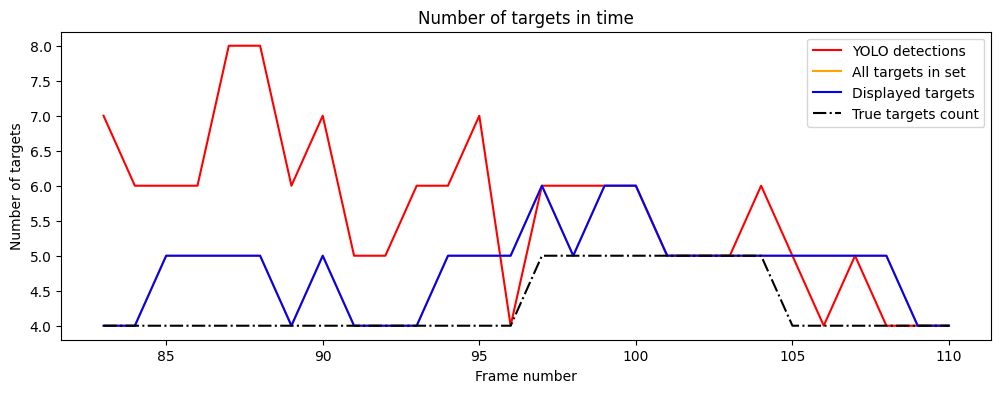
\includegraphics[width=\linewidth]{../../../experiments/\Ex/\Vs/SAM/sam_det}
    \caption{Development chart of the number of detected targets, targets in the filter's queue, displayed targets and
    true targets' count.}
    \label{gr:\Ex-\Vs-\Set}
\end{figure}

\begin{figure}[H]
    \centering
    \begin{subfigure}{0.23\textwidth}
        \centering
        \includegraphics[width=\linewidth]{../../../experiments/\Ex/\Vs/SAM/7}
        \caption{Frame number: 7}
        \label{fig:\Ex-\Vs-\Set:01}
    \end{subfigure}
    \begin{subfigure}{0.23\textwidth}
        \centering
        \includegraphics[width=\linewidth]{../../../experiments/\Ex/\Vs/SAM/33}
        \caption{Frame number: 33.}
        \label{fig:\Ex-\Vs-\Set:02}
    \end{subfigure}
    \begin{subfigure}{0.23\textwidth}
        \centering
        \includegraphics[width=\linewidth]{../../../experiments/\Ex/\Vs/SAM/38}
        \caption{Frame number: 38.}
        \label{fig:\Ex-\Vs-\Set:03}
    \end{subfigure}
    \begin{subfigure}{0.23\textwidth}
        \centering
        \includegraphics[width=\linewidth]{../../../experiments/\Ex/\Vs/SAM/43}
        \caption{Frame number: 43.}
        \label{fig:\Ex-\Vs-\Set:04}
    \end{subfigure}
    \\
    \begin{subfigure}{0.23\textwidth}
        \centering
        \includegraphics[width=\linewidth]{../../../experiments/\Ex/\Vs/SAM/57}
        \caption{Frame number: 57.}
        \label{fig:\Ex-\Vs-\Set:05}
    \end{subfigure}
    \begin{subfigure}{0.23\textwidth}
        \centering
        \includegraphics[width=\linewidth]{../../../experiments/\Ex/\Vs/SAM/60}
        \caption{Frame number: 60.}
        \label{fig:\Ex-\Vs-\Set:06}
    \end{subfigure}
    \begin{subfigure}{0.23\textwidth}
        \centering
        \includegraphics[width=\linewidth]{../../../experiments/\Ex/\Vs/SAM/85}
        \caption{Frame number: 85.}
        \label{fig:\Ex-\Vs-\Set:07}
    \end{subfigure}
    \begin{subfigure}{0.23\textwidth}
        \centering
        \includegraphics[width=\linewidth]{../../../experiments/\Ex/\Vs/SAM/92}
        \caption{Frame number: 92.}
        \label{fig:\Ex-\Vs-\Set:08}
    \end{subfigure}
    \caption{Image sequence of tracked objects using the GM-PHD filter with the dynamic detection probability, the YOLO
    object detector and the SAM image segmentation model.}
    \label{fig:\Ex-\Vs-\Set}
\end{figure}


\subsubsection{S3 -- Grounded SAM}
\renewcommand{\Set}{S3}
The combination of Grounding DINO and SAM is also evaluated on the video \textit{V3}. The utilized parameters are
outlined in Table \ref{tab:\Ex-\Vs-\Set}.
\begin{table}[H]
    \centering
    \begin{tabular}{|c|c|c|c|c|c|c|c|c|c|}
        \hline
        $P_{D,k}(x)$ & $P$ & $\sigma_{\upsilon}$ & $\sigma_{\epsilon}$ & $T_H$ & $T_d$ & $T_p$ & $T_l$ & $T_{text}$ & $T_{bbox}$\\ \noalign{\hrule
        height 1.5pt}
        0.3 & $diag(500,500,500,500)$ & 0.1 & 80 & 2 & 3 & 0.1 & 0.01 & 0.3 & 0.3\\
        \hline
    \end{tabular}
    \caption{The parameter settings for Experiment {\Ex-\Vs-\Set} with the dynamic detection probability.}
    \label{tab:\Ex-\Vs-\Set}
\end{table}

As seen in Figures \ref{fig:\Ex-\Vs-\Set:03}, \ref{fig:\Ex-\Vs-\Set:05} and \ref{fig:\Ex-\Vs-\Set:07}, Grounding DINO
is able to detect the hidden objects behind the light pole, thus the advantage of the dynamic detection probability is
not apparent. All targets are tracked precisely and no misdetection is present.

Till the frame no. 85, the number of displayed targets (blue line) and the number of targets in filter's queue (
orange line) exactly copies the true number of target's line in Graph \ref{gr:\Ex-\Vs-\Set}. It is, of course,
influenced
by the employment of the enhanced object detector, which has maneged to detect semi-hidden targets. The incresing and
decreasing number
of
targets after the frame 85 is due to the targets being close to each other.

\begin{figure}[H]
    \centering
    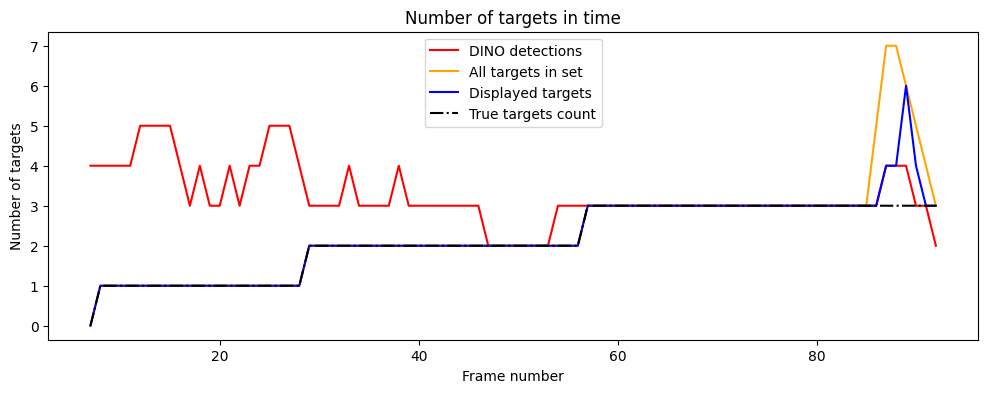
\includegraphics[width=\linewidth]{../../../experiments/\Ex/\Vs/DINO/dino_det}
    \caption{Development chart of the number of detected targets, targets in the filter's queue, displayed targets
    and true
    targets' count.}
    \label{gr:\Ex-\Vs-\Set}
\end{figure}

\begin{figure}[H]
    \centering
    \begin{subfigure}{0.23\textwidth}
        \centering
        \includegraphics[width=\linewidth]{../../../experiments/\Ex/\Vs/DINO/7}
        \caption{Frame number: 7.}
        \label{fig:\Ex-\Vs-\Set:01}
    \end{subfigure}
    \begin{subfigure}{0.23\textwidth}
        \centering
        \includegraphics[width=\linewidth]{../../../experiments/\Ex/\Vs/DINO/33}
        \caption{Frame number: 33.}
        \label{fig:\Ex-\Vs-\Set:02}
    \end{subfigure}
    \begin{subfigure}{0.23\textwidth}
        \centering
        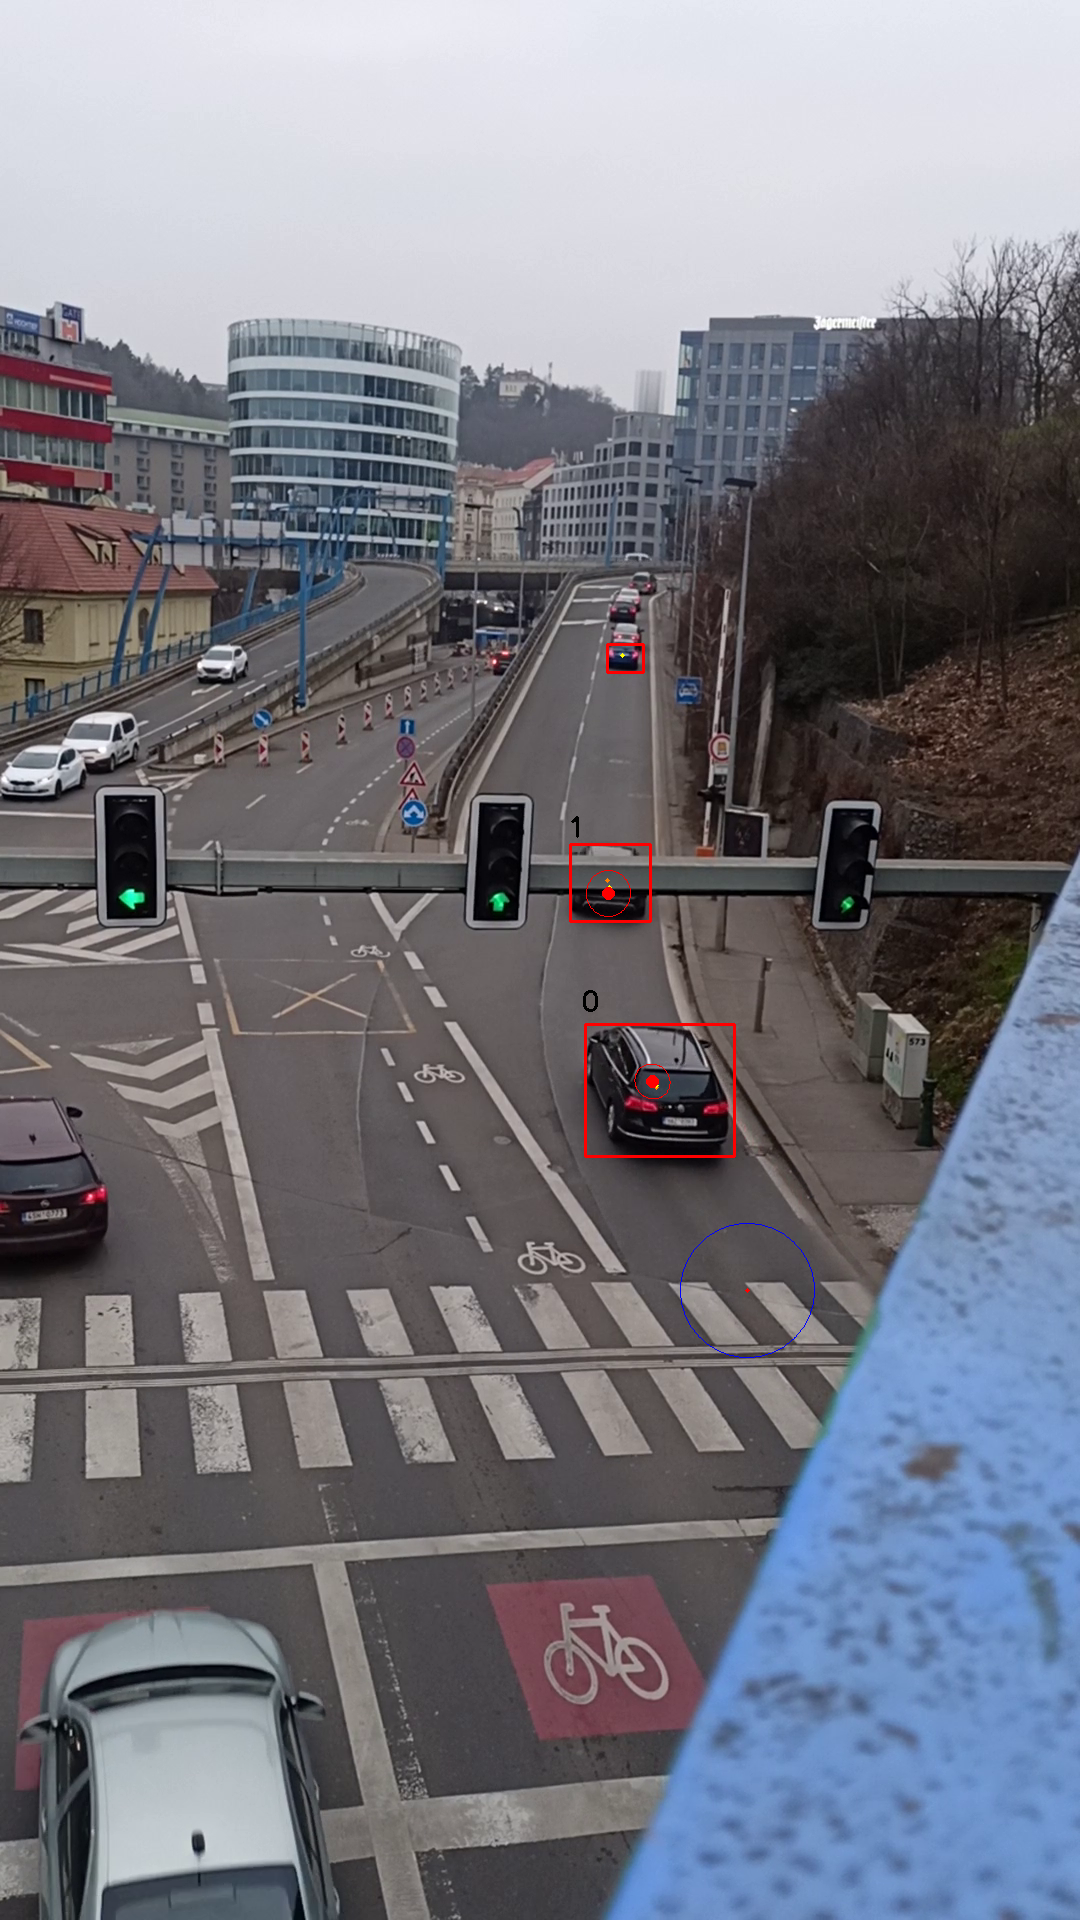
\includegraphics[width=\linewidth]{../../../experiments/\Ex/\Vs/DINO/39}
        \caption{Frame number: 39.}
        \label{fig:\Ex-\Vs-\Set:03}
    \end{subfigure}
    \begin{subfigure}{0.23\textwidth}
        \centering
        \includegraphics[width=\linewidth]{../../../experiments/\Ex/\Vs/DINO/43}
        \caption{Frame number: 43.}
        \label{fig:\Ex-\Vs-\Set:04}
    \end{subfigure}
    \\
    \begin{subfigure}{0.23\textwidth}
        \centering
        \includegraphics[width=\linewidth]{../../../experiments/\Ex/\Vs/DINO/57}
        \caption{Frame number: 57.}
        \label{fig:\Ex-\Vs-\Set:05}
    \end{subfigure}
    \begin{subfigure}{0.23\textwidth}
        \centering
        \includegraphics[width=\linewidth]{../../../experiments/\Ex/\Vs/DINO/60}
        \caption{Frame number: 60.}
        \label{fig:\Ex-\Vs-\Set:06}
    \end{subfigure}
    \begin{subfigure}{0.23\textwidth}
        \centering
        \includegraphics[width=\linewidth]{../../../experiments/\Ex/\Vs/DINO/85}
        \caption{Frame number: 85.}
        \label{fig:\Ex-\Vs-\Set:07}
    \end{subfigure}
    \begin{subfigure}{0.23\textwidth}
        \centering
        \includegraphics[width=\linewidth]{../../../experiments/\Ex/\Vs/DINO/92}
        \caption{Frame number: 92.}
        \label{fig:\Ex-\Vs-\Set:08}
    \end{subfigure}
    \caption{Image sequence of tracked objects using the GM-PHD filter with the dynamic detection probability, the DINO
    object detector and the SAM image segmentation model.}
    \label{fig:\Ex-\Vs-\Set}
\end{figure}




